\documentclass{standalone}
\usepackage{tikz}
\usetikzlibrary{patterns, positioning}

\begin{document}
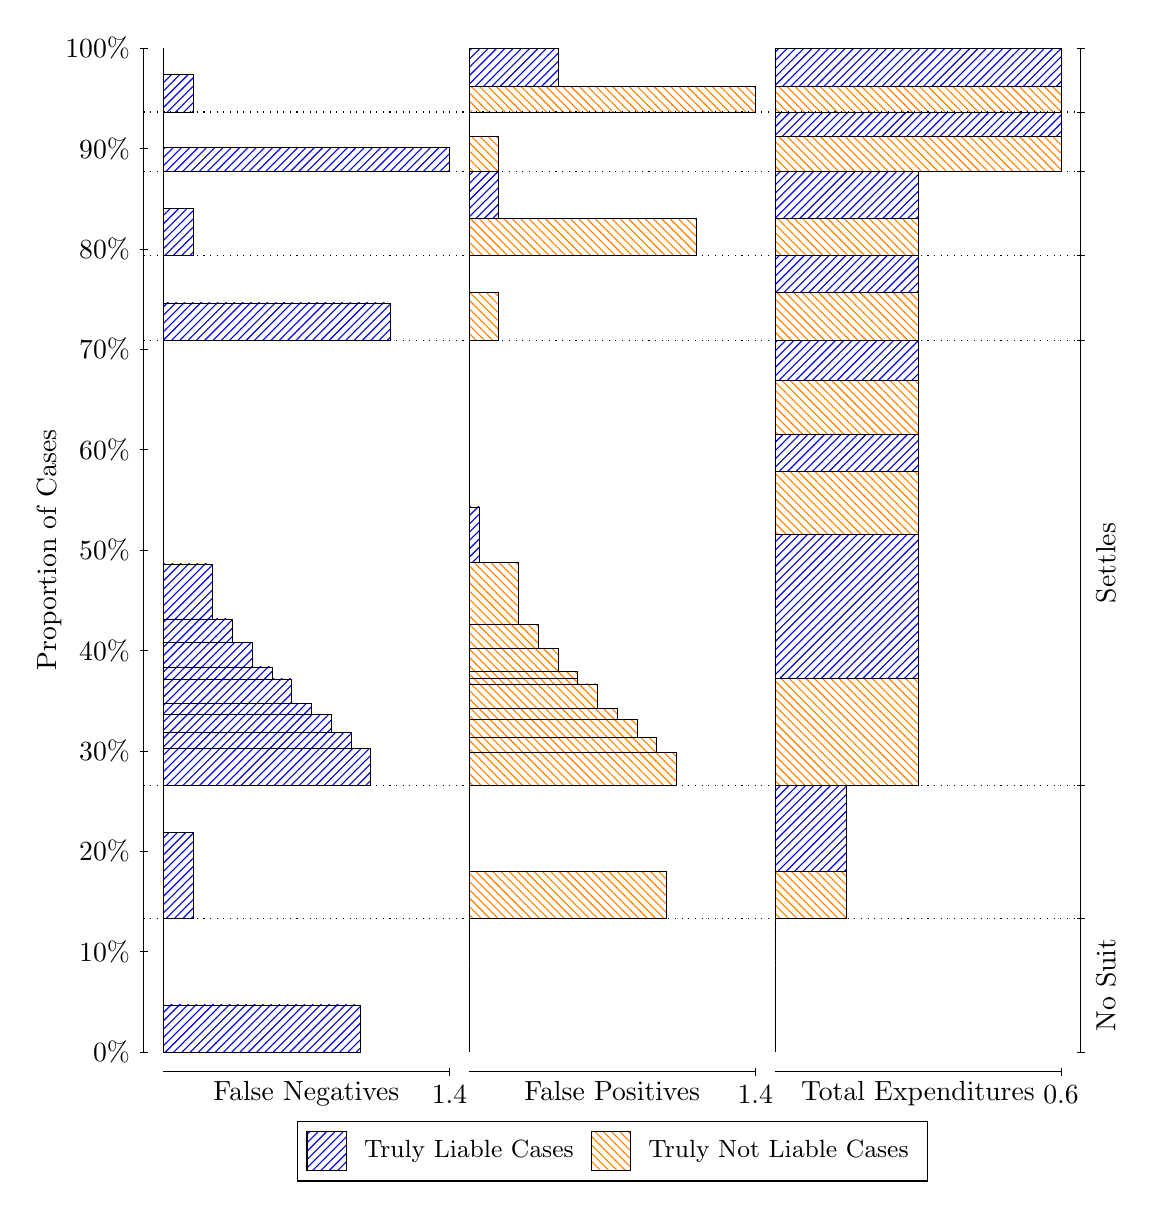
\begin{tikzpicture}
\draw[black, very thin] (1.5,1.75) -- (1.5,14.5);
\node[rotate=90, anchor=center] at (0.3, 8.125) {Proportion of Cases};
\draw[black, very thin] (1.45,1.75) -- (1.55,1.75);
\node[anchor=east] at (1.45, 1.75) {0\%};
\draw[black, very thin] (1.45,3.025) -- (1.55,3.025);
\node[anchor=east] at (1.45, 3.025) {10\%};
\draw[black, very thin] (1.45,4.3) -- (1.55,4.3);
\node[anchor=east] at (1.45, 4.3) {20\%};
\draw[black, very thin] (1.45,5.575) -- (1.55,5.575);
\node[anchor=east] at (1.45, 5.575) {30\%};
\draw[black, very thin] (1.45,6.85) -- (1.55,6.85);
\node[anchor=east] at (1.45, 6.85) {40\%};
\draw[black, very thin] (1.45,8.125) -- (1.55,8.125);
\node[anchor=east] at (1.45, 8.125) {50\%};
\draw[black, very thin] (1.45,9.4) -- (1.55,9.4);
\node[anchor=east] at (1.45, 9.4) {60\%};
\draw[black, very thin] (1.45,10.675) -- (1.55,10.675);
\node[anchor=east] at (1.45, 10.675) {70\%};
\draw[black, very thin] (1.45,11.95) -- (1.55,11.95);
\node[anchor=east] at (1.45, 11.95) {80\%};
\draw[black, very thin] (1.45,13.225) -- (1.55,13.225);
\node[anchor=east] at (1.45, 13.225) {90\%};
\draw[black, very thin] (1.45,14.5) -- (1.55,14.5);
\node[anchor=east] at (1.45, 14.5) {100\%};

\draw[black, very thin] (13.4,1.75) -- (13.4,14.5);
\draw[black, very thin] (13.35,1.75) -- (13.45,1.75);
\node[anchor=west] at (13.35, 1.75) {};
\draw[black, very thin] (13.35,3.4492) -- (13.45,3.4492);
\node[anchor=west] at (13.35, 3.4492) {};
\draw[black, very thin] (13.35,5.1319) -- (13.45,5.1319);
\node[anchor=west] at (13.35, 5.1319) {};
\draw[black, very thin] (13.35,10.788) -- (13.45,10.788);
\node[anchor=west] at (13.35, 10.788) {};
\draw[black, very thin] (13.35,11.869) -- (13.45,11.869);
\node[anchor=west] at (13.35, 11.869) {};
\draw[black, very thin] (13.35,12.931) -- (13.45,12.931);
\node[anchor=west] at (13.35, 12.931) {};
\draw[black, very thin] (13.35,13.687) -- (13.45,13.687);
\node[anchor=west] at (13.35, 13.687) {};
\draw[black, very thin] (13.35,14.5) -- (13.45,14.5);
\node[anchor=west] at (13.35, 14.5) {};

\draw[black, very thin, pattern color=blue, pattern=north east lines] (1.75,1.75) rectangle (4.2557,2.3488);
\draw[black, very thin, pattern color=orange, pattern=north west lines] (1.75,2.3488) rectangle (1.75,3.4492);
\draw[black, very thin, pattern color=blue, pattern=north east lines] (1.75,3.4492) rectangle (2.1259,4.5406);
\draw[black, very thin, pattern color=orange, pattern=north west lines] (1.75,4.5406) rectangle (1.75,5.1319);
\draw[black, very thin, pattern color=blue, pattern=north east lines] (1.75,5.1319) rectangle (4.381,5.6077);
\draw[black, very thin, pattern color=blue, pattern=north east lines] (1.75,5.6077) rectangle (4.1305,5.8081);
\draw[black, very thin, pattern color=blue, pattern=north east lines] (1.75,5.8081) rectangle (3.8799,6.0333);
\draw[black, very thin, pattern color=blue, pattern=north east lines] (1.75,6.0333) rectangle (3.6293,6.1745);
\draw[black, very thin, pattern color=blue, pattern=north east lines] (1.75,6.1745) rectangle (3.3787,6.4882);
\draw[black, very thin, pattern color=blue, pattern=north east lines] (1.75,6.4882) rectangle (3.1282,6.6408);
\draw[black, very thin, pattern color=blue, pattern=north east lines] (1.75,6.6408) rectangle (2.8776,6.9472);
\draw[black, very thin, pattern color=blue, pattern=north east lines] (1.75,6.9472) rectangle (2.627,7.2488);
\draw[black, very thin, pattern color=blue, pattern=north east lines] (1.75,7.2488) rectangle (2.3764,7.9499);
\draw[black, very thin, pattern color=orange, pattern=north west lines] (1.75,7.9499) rectangle (1.75,10.788);
\draw[black, very thin, pattern color=blue, pattern=north east lines] (1.75,10.788) rectangle (4.6316,11.262);
\draw[black, very thin, pattern color=orange, pattern=north west lines] (1.75,11.262) rectangle (1.75,11.869);
\draw[black, very thin, pattern color=blue, pattern=north east lines] (1.75,11.869) rectangle (2.1259,12.467);
\draw[black, very thin, pattern color=orange, pattern=north west lines] (1.75,12.467) rectangle (1.75,12.931);
\draw[black, very thin, pattern color=blue, pattern=north east lines] (1.75,12.931) rectangle (5.3833,13.243);
\draw[black, very thin, pattern color=orange, pattern=north west lines] (1.75,13.243) rectangle (1.75,13.687);
\draw[black, very thin, pattern color=blue, pattern=north east lines] (1.75,13.687) rectangle (2.1259,14.17);
\draw[black, very thin, pattern color=orange, pattern=north west lines] (1.75,14.17) rectangle (1.75,14.5);
\draw[black, very thin, pattern color=orange, pattern=north west lines] (5.6333,1.75) rectangle (5.6333,2.8504);
\draw[black, very thin, pattern color=blue, pattern=north east lines] (5.6333,2.8504) rectangle (5.6333,3.4492);
\draw[black, very thin, pattern color=orange, pattern=north west lines] (5.6333,3.4492) rectangle (8.1391,4.0405);
\draw[black, very thin, pattern color=blue, pattern=north east lines] (5.6333,4.0405) rectangle (5.6333,5.1319);
\draw[black, very thin, pattern color=orange, pattern=north west lines] (5.6333,5.1319) rectangle (8.2644,5.5509);
\draw[black, very thin, pattern color=orange, pattern=north west lines] (5.6333,5.5509) rectangle (8.0138,5.7477);
\draw[black, very thin, pattern color=orange, pattern=north west lines] (5.6333,5.7477) rectangle (7.7632,5.978);
\draw[black, very thin, pattern color=orange, pattern=north west lines] (5.6333,5.978) rectangle (7.5126,6.1125);
\draw[black, very thin, pattern color=orange, pattern=north west lines] (5.6333,6.1125) rectangle (7.2621,6.4244);
\draw[black, very thin, pattern color=orange, pattern=north west lines] (5.6333,6.4244) rectangle (7.0115,6.4931);
\draw[black, very thin, pattern color=orange, pattern=north west lines] (5.6333,6.4931) rectangle (7.0115,6.5817);
\draw[black, very thin, pattern color=orange, pattern=north west lines] (5.6333,6.5817) rectangle (6.7609,6.8745);
\draw[black, very thin, pattern color=orange, pattern=north west lines] (5.6333,6.8745) rectangle (6.5103,7.1762);
\draw[black, very thin, pattern color=orange, pattern=north west lines] (5.6333,7.1762) rectangle (6.2598,7.9701);
\draw[black, very thin, pattern color=blue, pattern=north east lines] (5.6333,7.9701) rectangle (5.7586,8.6712);
\draw[black, very thin, pattern color=blue, pattern=north east lines] (5.6333,8.6712) rectangle (5.6333,10.788);
\draw[black, very thin, pattern color=orange, pattern=north west lines] (5.6333,10.788) rectangle (6.0092,11.396);
\draw[black, very thin, pattern color=blue, pattern=north east lines] (5.6333,11.396) rectangle (5.6333,11.869);
\draw[black, very thin, pattern color=orange, pattern=north west lines] (5.6333,11.869) rectangle (8.5149,12.333);
\draw[black, very thin, pattern color=blue, pattern=north east lines] (5.6333,12.333) rectangle (6.0092,12.931);
\draw[black, very thin, pattern color=orange, pattern=north west lines] (5.6333,12.931) rectangle (6.0092,13.375);
\draw[black, very thin, pattern color=blue, pattern=north east lines] (5.6333,13.375) rectangle (5.6333,13.687);
\draw[black, very thin, pattern color=orange, pattern=north west lines] (5.6333,13.687) rectangle (9.2667,14.016);
\draw[black, very thin, pattern color=blue, pattern=north east lines] (5.6333,14.016) rectangle (6.7609,14.5);
\draw[black, very thin, pattern color=orange, pattern=north west lines] (9.5167,1.75) rectangle (9.5167,2.8504);
\draw[black, very thin, pattern color=blue, pattern=north east lines] (9.5167,2.8504) rectangle (9.5167,3.4492);
\draw[black, very thin, pattern color=orange, pattern=north west lines] (9.5167,3.4492) rectangle (10.425,4.0405);
\draw[black, very thin, pattern color=blue, pattern=north east lines] (9.5167,4.0405) rectangle (10.425,5.1319);
\draw[black, very thin, pattern color=orange, pattern=north west lines] (9.5167,5.1319) rectangle (11.333,6.4931);
\draw[black, very thin, pattern color=blue, pattern=north east lines] (9.5167,6.4931) rectangle (11.333,8.3274);
\draw[black, very thin, pattern color=orange, pattern=north west lines] (9.5167,8.3274) rectangle (11.333,9.1212);
\draw[black, very thin, pattern color=blue, pattern=north east lines] (9.5167,9.1212) rectangle (11.333,9.597);
\draw[black, very thin, pattern color=orange, pattern=north west lines] (9.5167,9.597) rectangle (11.333,10.28);
\draw[black, very thin, pattern color=blue, pattern=north east lines] (9.5167,10.28) rectangle (11.333,10.788);
\draw[black, very thin, pattern color=orange, pattern=north west lines] (9.5167,10.788) rectangle (11.333,11.396);
\draw[black, very thin, pattern color=blue, pattern=north east lines] (9.5167,11.396) rectangle (11.333,11.869);
\draw[black, very thin, pattern color=orange, pattern=north west lines] (9.5167,11.869) rectangle (11.333,12.333);
\draw[black, very thin, pattern color=blue, pattern=north east lines] (9.5167,12.333) rectangle (11.333,12.931);
\draw[black, very thin, pattern color=orange, pattern=north west lines] (9.5167,12.931) rectangle (13.15,13.375);
\draw[black, very thin, pattern color=blue, pattern=north east lines] (9.5167,13.375) rectangle (13.15,13.687);
\draw[black, very thin, pattern color=orange, pattern=north west lines] (9.5167,13.687) rectangle (13.15,14.016);
\draw[black, very thin, pattern color=blue, pattern=north east lines] (9.5167,14.016) rectangle (13.15,14.5);
\draw[black, dotted] (1.5,3.4492) -- (13.4,3.4492);
\draw[black, dotted] (1.5,5.1319) -- (13.4,5.1319);
\draw[black, dotted] (1.5,10.788) -- (13.4,10.788);
\draw[black, dotted] (1.5,11.869) -- (13.4,11.869);
\draw[black, dotted] (1.5,12.931) -- (13.4,12.931);
\draw[black, dotted] (1.5,13.687) -- (13.4,13.687);
\draw[black, very thin] (1.75,1.5) -- (5.3833,1.5);
\node[anchor=north] at (3.5667, 1.5) {False Negatives};
\draw[black, very thin] (5.3833,1.45) -- (5.3833,1.55);
\node[anchor=north] at (5.3833, 1.45) {1.4};

\draw[black, very thin] (5.6333,1.5) -- (9.2667,1.5);
\node[anchor=north] at (7.45, 1.5) {False Positives};
\draw[black, very thin] (9.2667,1.45) -- (9.2667,1.55);
\node[anchor=north] at (9.2667, 1.45) {1.4};

\draw[black, very thin] (9.5167,1.5) -- (13.15,1.5);
\node[anchor=north] at (11.333, 1.5) {Total Expenditures};
\draw[black, very thin] (13.15,1.45) -- (13.15,1.55);
\node[anchor=north] at (13.15, 1.45) {0.6};

\node[black, centered, rotate=90] at (13.72, 2.5996) {No Suit};

\node[black, centered, rotate=90] at (13.72, 7.96) {Settles};





\draw (7.449999999999999,1.5) node[draw=none] (baseCoordinate) {};
\begin{scope}[align=center]
        \matrix[scale=0.5, draw=black, below=0.5cm of baseCoordinate, nodes={draw}, column sep=0.1cm]{
            \node[rectangle, draw, minimum width=0.5cm, minimum height=0.5cm, pattern=north east lines, pattern color=blue] {}; &
            \node[draw=none, font=\small] (B) {Truly Liable Cases}; &
            \node[rectangle, draw, minimum width=0.5cm, minimum height=0.5cm, pattern=north west lines, pattern color=orange] {}; &
            \node[draw=none, font=\small] (B) {Truly Not Liable Cases}; \\
            };
\end{scope}

\end{tikzpicture}
\end{document}